\section{Adjoint-flux compression for weight-window storage}
\label{sec:adjoint-compression}

The same SVD machinery used for cross-section compression
(Section~\ref{sec:method}) applies — with a one-line code change — to
the random-ray adjoint flux $\psi^{*}(\mathbf{r}, g)$ used by FW-CADIS
weight-window generation~\citep{evans2020adjoint}. The adjoint
solver returns $\psi^{*}$ as a row-major
$[n_{\text{FSR}} \times n_{g}]$ matrix; for Cartesian voxel meshes
this reshapes naturally as
$[n_{x}\,n_{y} \times n_{z}]$, separating the streaming axis from the
transverse plane. Slab and duct geometries put almost all of
$\psi^{*}$ in a single dominant singular triplet of this reshape,
leaving the rest of the spectrum to capture statistical noise from
the MC adjoint solve.

\subsection{Adaptive picker}

Rather than picking a fixed rank, the implementation uses an
adaptive picker: given a Frobenius reconstruction tolerance
$\varepsilon$, return the lowest-rank SVD whose linear-space
reconstruction satisfies $\|\hat\psi^{*} - \psi^{*}\|_{F} /
\|\psi^{*}\|_{F} \le \varepsilon$ and whose factored byte count
$(m + n + 1) \cdot k \cdot 8$ is strictly below the dense baseline
$m \cdot n \cdot 8$. If no rank in $1 \ldots k_{\max}$ qualifies,
the picker falls back to the dense matrix. Both linear-space and
$\log_{10}$-space SVD are tried; the smaller representation that
meets $\varepsilon$ wins. The dense fallback is byte-identical to
the existing CADIS map JSON the photon-side weight-window pipeline
already consumes, so the switch is invisible to downstream code.

\subsection{Mesh-size sweep}

A meaningful sweep needs the voxels to be coarser than the
underlying physics: subdividing finer than $\sim$mfp/8 introduces
no signal, only noise from the random-ray sampling. For water at
1\,MeV (mfp $\approx 14$\,cm) the floor is $\approx 1.77$\,cm,
so the sweep is restricted to meshes whose smallest voxel edge is
$\ge$ mfp/8. The sweep binary refuses sub-mfp meshes at the
source so that pollution can't sneak into the analysis.

Figure~\ref{fig:adjoint-compression} runs 23 such meshes through
the picker at two Frobenius tolerances. Voxel counts span 25 to
$1.25 \times 10^{5}$ — a 3.7-decade range bounded above by the
physics-resolution floor. Numbers are \texttt{[micro]}-scope —
they characterise the compression kernel on real solver output,
not end-to-end shielding tally throughput. Random-ray statistics
are fixed at $200 \times 8000$ rays for every mesh.

\begin{figure*}[t]
  \centering
  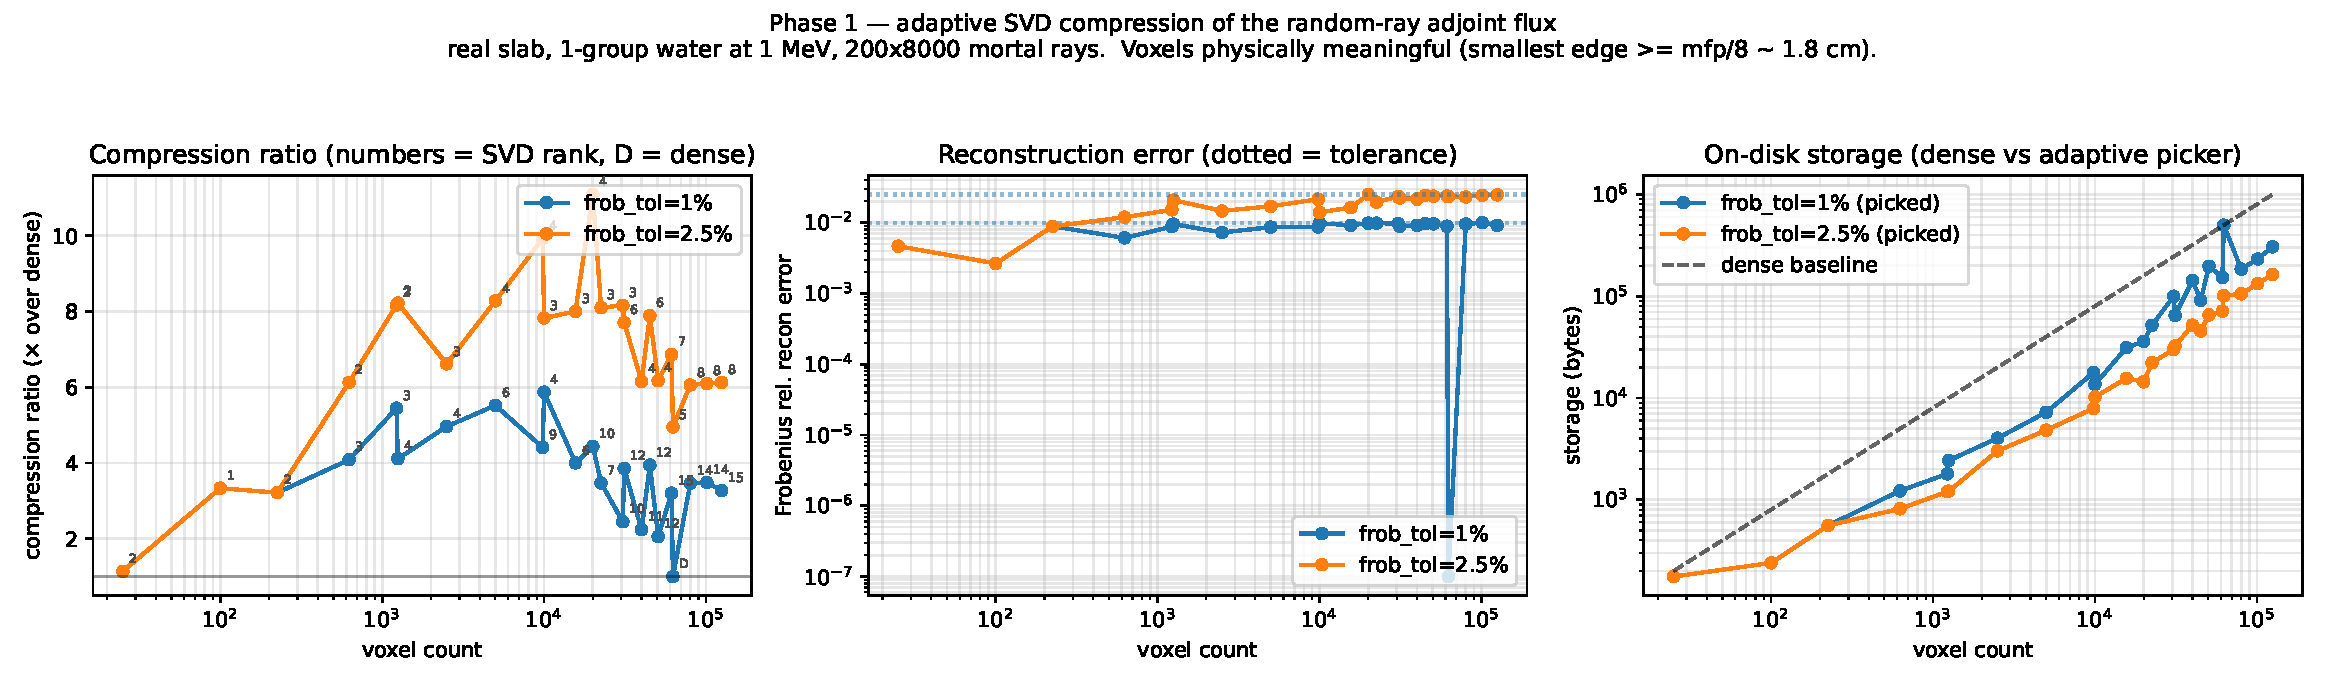
\includegraphics[width=\linewidth]{figures/adjoint_compression}
  \caption{%
    Adaptive SVD compression of the random-ray adjoint flux on the
    slab benchmark, water at 1\,MeV, 1-group, mortal rays
    ($200\times 8000$). 23 mesh configurations restricted to
    physically meaningful voxel resolutions
    (smallest edge $\ge$ mfp/8 $\approx$ 1.77\,cm); voxel counts
    span 25 to $1.25\times 10^{5}$. Annotations are SVD rank
    chosen (\texttt{D} = dense fallback).
    \emph{Left}: compression ratio at $\varepsilon=2.5\%$ rises to
    $\sim$8--11$\times$ between $10^{3}$ and $10^{5}$ voxels and
    stays in that band; the peak is $11.09\times$ at
    $20\times20\times50 = 20\,000$ voxels.
    \emph{Middle}: linear reconstruction error stays under the
    requested tolerance band on every retained SVD pick; dense
    fallbacks are off-scale (exact, plotted at the $\varepsilon$
    floor).
    \emph{Right}: storage in bytes — picked vs dense.}
  \label{fig:adjoint-compression}
\end{figure*}

\begin{table}[t]
  \centering
  \small
  \begin{tabular}{l r r r l r}
    \toprule
    mesh & voxels & dense & $\varepsilon$ & picked & ratio \\
    \midrule
    \multicolumn{6}{l}{\emph{$\varepsilon = 2.5\%$ — selected sweep points}} \\
    $1\!\times\!1\!\times\!25$       & 25       & 200\,B    & 2.5\,\% & $k{=}2$ & $1.14\times$ \\
    $5\!\times\!5\!\times\!25$       & 625      & 5.0\,KB   & 2.5\,\% & $k{=}2$ & $6.13\times$ \\
    $10\!\times\!10\!\times\!25$     & 2\,500   & 20\,KB    & 2.5\,\% & $k{=}3$ & $6.61\times$ \\
    $20\!\times\!20\!\times\!50$     & 20\,000  & 156\,KB   & 2.5\,\% & $k{=}4$ & $\mathbf{11.09\times}$ \\
    $30\!\times\!30\!\times\!25$     & 22\,500  & 176\,KB   & 2.5\,\% & $k{=}3$ & $8.10\times$ \\
    $35\!\times\!35\!\times\!25$     & 30\,625  & 239\,KB   & 2.5\,\% & $k{=}3$ & $8.16\times$ \\
    $30\!\times\!30\!\times\!50$     & 45\,000  & 351\,KB   & 2.5\,\% & $k{=}6$ & $7.89\times$ \\
    $50\!\times\!50\!\times\!25$     & 62\,500  & 488\,KB   & 2.5\,\% & $k{=}5$ & $4.95\times$ \\
    $40\!\times\!40\!\times\!50$     & 80\,000  & 625\,KB   & 2.5\,\% & $k{=}8$ & $6.06\times$ \\
    $50\!\times\!50\!\times\!50$     & 125\,000 & 977\,KB   & 2.5\,\% & $k{=}8$ & $6.13\times$ \\
    \midrule
    \multicolumn{6}{l}{\emph{$\varepsilon = 1.0\%$ — selected sweep points}} \\
    $5\!\times\!5\!\times\!25$       & 625      & 5.0\,KB   & 1.0\,\% & $k{=}3$ & $4.09\times$ \\
    $20\!\times\!20\!\times\!50$     & 20\,000  & 156\,KB   & 1.0\,\% & $k{=}10$ & $4.43\times$ \\
    $30\!\times\!30\!\times\!25$     & 22\,500  & 176\,KB   & 1.0\,\% & $k{=}7$ & $3.47\times$ \\
    $40\!\times\!40\!\times\!50$     & 80\,000  & 625\,KB   & 1.0\,\% & $k{=}14$ & $3.46\times$ \\
    $50\!\times\!50\!\times\!50$     & 125\,000 & 977\,KB   & 1.0\,\% & $k{=}15$ & $3.27\times$ \\
    $50\!\times\!50\!\times\!25$     & 62\,500  & 488\,KB   & 1.0\,\% & dense    & $1.00\times$ \\
    \bottomrule
  \end{tabular}
  \caption{Picker decisions on the 23-mesh physics-respecting
    sweep (smallest voxel edge $\ge$ mfp/8 $\approx$ 1.77\,cm),
    slab benchmark, $200\times 8000$ mortal rays. Selected rows;
    full data in
    \texttt{outputs/adjoint\_sweep\_valid\_tol\{1,2.5\}pct.csv}.
    At $\varepsilon=2.5\%$ every mesh in the meaningful range
    compresses, in a $5{-}11\times$ band. Tightening to
    $\varepsilon=1\%$ shrinks the picked rank's headroom and
    flips a few of the largest meshes to the dense fallback.}
  \label{tab:adjoint-picker-sweep}
\end{table}

The compression ratio rises with mesh size as the picker fills
out the rank-1 dominant streaming mode and stabilises in a
$\sim 5{-}11\times$ band once the mesh is large enough to
saturate that mode. At $\varepsilon=2.5\%$ every mesh in the
physically meaningful range compresses; the picker chooses ranks
that grow gradually with voxel count (typically $k{=}2{-}8$).
At $\varepsilon=1\%$ the picker still wins on most meshes but
falls back to dense at $50\!\times\!50\!\times\!25$ — the
random-ray noise floor at 200\,$\times$\,8000 rays catches up
with the tolerance there. In a deployment scenario the picker
simply picks the rank that satisfies the user's accuracy budget
or returns dense — there is no manual tuning and no risk of a
silent accuracy regression. For the existing
\texttt{outputs/cadis\_water\_*.json} files
($1\!\times\!1\!\times\!n_z$ mesh, $n_z \le 25$) the picker
chooses dense or a small rank-2 SVD with $\sim 1.1\times$
savings; the win arrives only when 3D voxelisation is enabled,
as the literature predicted, and grows to the $5{-}11\times$
band across the meshes where $\psi^{*}$ compression actually
matters for storage budgets.

Sub-mfp meshes were tried during exploration but produce no
meaningful result — the geometric subdivision is finer than the
random-ray sampling can resolve, so the picker is forced to fit
noise. The sweep binary refuses sub-mfp meshes at the source
(asserting that the smallest voxel edge be $\ge$ mfp/8) so that
the analysis cannot be polluted by configurations where the
physics carries no signal.

\subsection{Approaches that did not pan out}
\label{subsec:adjoint-negatives}

Two alternative compression strategies were implemented and
benchmarked against the SVD picker, but neither displaced it.

\paragraph{Tensor-train decomposition.}
The 3-tensor $\Sigma(E, T, R)$ for a single nuclide can in principle
be compressed jointly via TT-SVD~\citep{oseledets2011tt} rather than
per-reaction 2D SVD. On a synthetic
$5000 \times 9 \times 52$ tensor with planted CP-rank 5, TT at rank
$(5,5)$ used $51\times$ less memory than the per-reaction baseline
and matched it on accuracy. On real U-235 data with
$3000 \times 6 \times 6$ (six reactions), TT at rank 5 was
$6\times$ smaller but $\approx 10^{3}\times$ less accurate than
the production per-reaction 2D SVD at the same nominal rank
($4.8 \times 10^{-3}$ vs $4.2 \times 10^{-6}$ Frobenius rel error).
TT loses one degree of freedom in the joint structure, and on the
small reaction counts and high accuracy budgets relevant to MC
$k_{\text{eff}}$ that loss is not tradeable for the memory win.
This is consistent with the prior cross-isotope basis-sharing
result (subspace angle $> 85^{\circ}$ at $k=2$) but rules out a
stronger method as well.

\paragraph{Discrete cosine transform of $\sigma(E,T)$.}
A 2D DCT-II of $\log\sigma(E,T)$ truncated to the top-$K$
coefficients was benchmarked head-to-head against SVD on
U-235 fission MT~18 across five byte budgets from 8\,KB to
128\,KB. SVD won at every budget tested. Off-library
reconstruction at $T_{\text{q}} = 750\,\mathrm{K}$ (between the
600\,K and 900\,K library columns) gave SVD $4.7 \times 10^{-3}$
relative error at 16\,KB while DCT achieved
$2.1 \times 10^{-2}$; at 128\,KB SVD becomes machine-exact while
DCT remains at $1.7 \times 10^{-3}$. The off-library memory edge
of SVD reported in
Section~\ref{sec:memprec} is therefore not eliminated by a clean
transform-and-truncate alternative. A heat-equation
formulation~\citep{ducru2017} of DCT-DB might do
better, but at WMP-scale implementation effort this was not in
scope; the simple alternative is dominated.

The full benchmark CSVs and numbers for both negative results live
at \texttt{outputs/phase2\_tt\_decompose.txt} and
\texttt{outputs/phase3\_dct\_db.txt}.
